\documentclass[11pt,a4paper]{amsart}
\usepackage{amsmath,amsthm,amssymb}
\usepackage{parskip}
\usepackage{listings}
\lstloadlanguages{R}
\usepackage{verbatim}
\usepackage[usenames,dvipsnames]{color}
\usepackage{esdiff}
\usepackage{subfig}
\lstset{
   language=R,
   basicstyle=\ttfamily,
   columns=fixed,
   fontadjust=true,
   breaklines=true,
   basewidth=0.5em,
   keywordstyle=\color{blue},
   commentstyle=\color{ForestGreen},
   stringstyle=\color{mauve}
}
\fontfamily{cmr}
\usepackage[margin=1in, tmargin=0.75in, bmargin=0.75in]{geometry}
\usepackage{graphicx}
\usepackage{enumerate}
\title{MAS212 Assignment 2:\\The Van der Pol oscillator}
\author{140185164}
\begin{document}

\maketitle

Balthasar Van der Pol was  a physicist and electrical engineer who specialised in the study of radio communications. Whilst Van der Pol was working for Philips in Holland, he studied the vacuum tubes that were used to regulate electric current flow to transmitters and receivers in radios.$^{[1]}$ Van der Pol's research took on a life of its own, other scientists contributed their research and discovered that many of the oscillating circuits could be modelled by second-order differential equations of the form $$\ddot{x} +f(x)\dot{x}+g(x)=0.$$
This is now known as Lienard's equation. If we let $f(x)=-a(1-x^2)$ then, we have a special case of Lienard's equation, known famously as the Van der Pol equation: $$\ddot{x} -a(1-x^2)\dot{x} + x =0.^{[2]}$$\par
%There exists a theorem, called Lienard's theorem, which states that if 5 conditions (existing on $f$ and $g$) hold on a Lienard equation, then the equation has a unique stable limit cycle surrounding the origin.$^{[3]}$ The \textit{undriven} Van der Pol oscillator satisfies the conditions stated in Lienard's equation.  
The \textit{undriven} Van der Pol oscillator can be adapted to incorporate a \textit{driving} term, giving us the following general Van der Pol oscillator:
\begin{equation}\ddot{x} -a(1-x^2)\dot{x} + x =b\cos(\omega t),\ a,b,\omega\in\mathbb{R}.\end{equation}

\subsection*{Derivation of some key results}Second order differential equations can be broken down into a system of first order differential equations, and the Van der Pol equation makes no exception. If we let $\dot{x}=y,$ then $\diff{}{x}y=\dot{y}=\diff{}{x}\dot{x}=\ddot{x}.$ Now we notice that $\dot{y}=\ddot{x}=a(1-x^2)\dot{x}-x+b\cos(\omega t)$ by making $\ddot{x}$ the subject of the Van der Pol equation. Finally, substituting $y$ for $\dot{x}$ in $\dot{y}$ gives:
\begin{align} 
\dot{x}=&y \nonumber \\
\dot{y}=&a(1-x^2)y-x+b\cos(\omega t).
\end{align}

In the undamped, undriven case (where $a=0,$ $b=0$), we have $\dot{y}=-x.$ We need to show by back-substitution that the general solution for equation (2) is: 
$$
x=\alpha\cos(t+\beta),\ y={-\alpha\sin(t+\beta)}.$$
We will show that the right-hand side and left-hand side (RHS and LHS respectively) of (2) are equal to eachother. So, 
\begin{align*}
\text{RHS}&={-x}={-\alpha\cos(t+\beta)},\\
\text{and}\  \text{LHS} &=  \dot{y}=\diff{}{t}y=\diff{}{t}{-\alpha\sin(t+\beta)}= {-\alpha\cos(t+\beta)}.
\end{align*}
 \\It is clear that $\text{LHS}=\text{RHS}={-\alpha}\cos(t+\beta),$ hence the equation holds for $x$ and $y$, and so $x$ and $y$ give the general solution for $(2).$
It is interesting to note that in this case, when $a=b=0$, the differential equation is one that models \textit{simple harmonic motion}.
\subsection*{The driven oscillator}
We will now consider the undamped oscillator, where $a=0$, $b\neq0$. If we insert the given periodic solution into $(2)$ we get:
\begin{align*}
\dot{y} = \diff{}{t} [{-A}\omega\sin(\omega t)]={-A}\cos(\omega t)+b\cos(wt) \\ 
\iff {-A}\omega^2\cos(\omega t)={-A}\cos(\omega t)+b\cos(wt).
\end{align*}

There are now two possibilities. Either $\cos(\omega t) = 0 \iff \omega t=2k\pi$ for some $k\in\mathbb{R}$, or $\cos(\omega t) \neq 0$. If we take $\cos(\omega t) = 0$ we get $0=0+0$ (trivial solution) and so we will consider $\cos(\omega t)\neq 0.$ Since $\cos(\omega t) \neq 0$ we can divide through our equation by it giving $${-A}\omega^2={-A}+b\iff A(1-\omega^2)=b \iff A=\frac{b}{1-\omega^2}.$$
A is the amplitude of the oscillator and it is a function of $b$ and $\omega$ only, making it \textit{time-independent}. We now consider the following limit: $\lim_{\omega \to 1} A = \lim_{\omega \to 1} \frac{b}{1-\omega^2} =\infty.$ This tells us that as $\omega$ gets closer to $1$, $\frac{b}{1-\omega^2}$ gets larger and larger. Since division by $0$ is undefined, $\omega \neq 1$.
\\
%%insert explaination of what this means for this periodic solution.

\section*{The undriven Van der Pol oscillator}
I will begin by exploring the undriven (yet dampened) oscillator, which is given by $$\ddot{x}-a(1-x^2)\dot{x}+x=0.$$ This is a non-linear ODE and so no analytical solution can be found. Instead we can find numerical solutions for the ODE over a given time-domain, and then plot a graph to show how $x$ varies over time $t$. We were tasked with plotting the dampened ODE over a given time-domain for various initial conditions $x_{0}$ and $\dot{x}_{0}\ (=y_0)$. This is illustrated in the graph below:

\begin{figure}[h]
\caption{Solutions of the undriven Van der Pol oscillator, with parameters $a=\frac{1}{2}$, $b=0$, and initial conditions $x_0=\{0.1,1,2,3\}$ and $y_0=0$.}
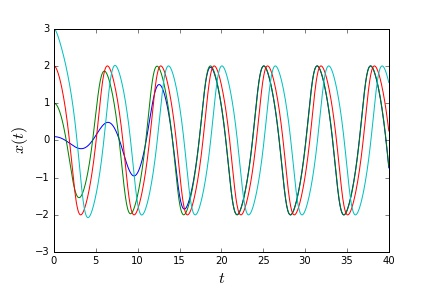
\includegraphics[scale=0.6]{part_2a.jpg}
\centering
\end{figure}

We can see from Figure 1 that the the curve with initial condition $x_0=0.1$ starts off with week oscillations compared to curves for $x0=\{1,2,3\}$, but, after approximately 15 seconds, has the same range of $x(t)$ values as the other three curves. We can also see that each curve is periodic, and also if the initial condition $x_0$ is larger, it appears that it is translated along the ${x-}$axis. We could theorise from this plot that for some initial conditions $x_{0b}>x_{0a}$, once the oscillations stabilise for both curves, say at time $t=T$, then the curve $x_{0b}$ is a translation of the curve $x_{0a}$ along the positive ${x-}$axis for $t\in(T,\infty)$. 

It can also be insightful to consider the phase plot as well as the time-domain plot in Figure 1. Using the same parameters as in Figure 1, we can plot the corresponding phase plot: 

\begin{figure}[h]
\caption{Plots investigating the effect of change in initial conditions on the phase portrait composition (A), and the effect of changing the value of $a$ on the shape of the limit cycle (B).}
\centering
\subfloat[Phase-plot of the undriven Van der Pol oscillator, with parameters $a=\frac{1}{2}$, $b=0$, and initial conditions $x_0=\{0.1,1,2,3\}$ and $y_0=0$.]{
	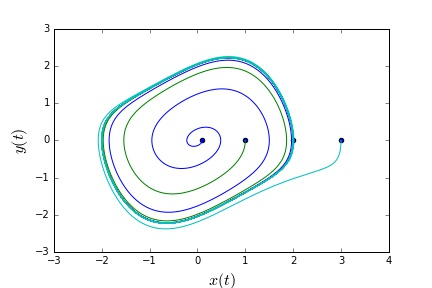
\includegraphics[scale=0.5]{part_2b.jpg}
	\label{fig:sub1}
	}
	\hfill
\subfloat[Limit cycles of the undriven Van der Pol equation for $a=\{0.1,1,2,3\}$, and initial conditions $x_0=3$, $y_0=0$.]{
	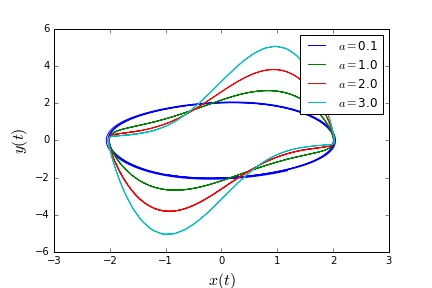
\includegraphics[scale=0.5]{part_2c.jpg}
	\label{fig:sub2}
	}
\end{figure}

The end points of each curve on the plot represents the initial conditions for each curve. As you follow each curve around the plot, we can see that the curves tend closer and closer to each other, indicative of something known as a \textit{limit cycle}. A \textit{limit cycle} is a cycle for which trajecories converge to in a system of ODEs.

If we fix one $x_0$ and one $y_0$, and allow $a$ to vary in the Van der Pol equation, we can see how limit cycles vary for different values of $a$. In our next model, we chose $a=\{0.1,1,2,3\}$ and then plotted a graph of $x$ against $y$. However, we only plot the graph between $t\in[20,40]$ so that the curves have had chance to converge to their respective limit cycles.

As $a$ increases, the limit cycle stretches and becomes increasingly distorted parallel to the ${y(t)-}$ axis.

\section*{The driven oscillator}
In this section we will consider the Van der pol equation with $b\neq0$. Below are two figures corresponding to a time-domain plot and a phase plot for parameters $a=3,\ b=5$ and $\omega=1.788$.

\begin{figure}[h]
\caption{Time-domain plot (\textit{left}) and phase plot (\textit{right}) for the driven oscillator using the given parameters}
\centering
\subfloat[Time-domain graph]{
	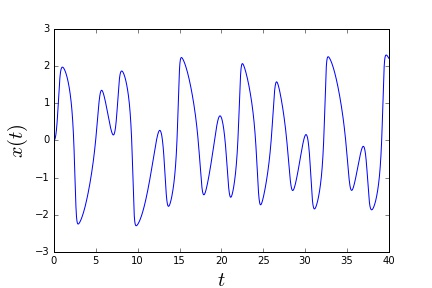
\includegraphics[scale=0.45]{part_3a.jpg}
	\label{fig:sub1}
	}
	\hfill
\subfloat[Phase portrait]{
	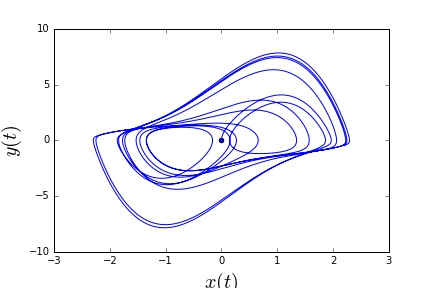
\includegraphics[scale=0.45]{part_3a_2.jpg}
	\label{fig:sub2}
	}
\end{figure}

By inspecting the time-domain graph we can see that the response is not periodic for the region $t\in[0,40]$. Also, if we inspect the phase portrait, for small $t$ we can see that instead the trajectory tending to a limit cycle rather quickly, the trajectory oscillates in roughly the shape of $\infty$, until eventually the trajectory converges roughly to the shape of the limit cycle of the undriven Van der Pol oscillator for $a=3$.

\subsection*{Poincar\'e sections}Poincar\'e sections, or surface of sections, are graphs in which only points that trigger a particular condition are plotted. In our poincar\'e section, the condition on the Van der Pol equation is that all points $(x(t_k),y(t_k))$ are plotted for $t_k=\frac{2\pi k}{\omega}$, where $500\leq k \leq 5000$ are integers. 

Since $\cos(\omega t_k)=\cos\big(\omega\frac{2\pi k}{\omega}\big) =\cos(2\pi k)=1,\  \forall k\in \mathbb{Z}$, we have the following trigger:
$$\ddot{x}_{t_k} -3(1-x_{t_k}^2)\dot{x}_{t_k} + x_{t_k} =5\cos(\omega t_k)=5.$$ 

\begin{figure}[h]
\caption{Poincar\'e section plotting $x(t_k)$ against $y(t_k)$ for the above parameters}
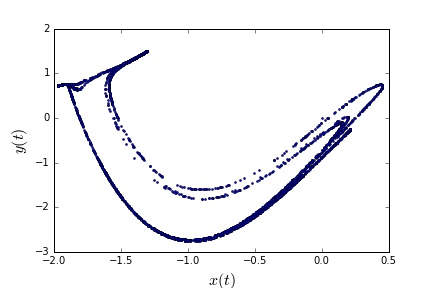
\includegraphics[scale=0.5]{part_3b.jpg}
\centering
\end{figure}

The points plotted on the graph above start by occuring a fair way apart from each other, then gradually get nearer and nearer, indicating that the points are tending to a particular $(x,y)$, and upon inspection of the final point plotted on the graph, we see that $(x_{t_{5000}},y_{t_{5000}})=(4.99999,6.9068\times 10^{-13}) \approx (5,0)$. I would conclude from this inspection that as $k\to\infty$, $(x_{t_k},y_{t_k}) \to (5,0)$.

\subsection*{Strange attractors} A very intuitive and concise definition for a strange attractor is as follows:\\
\textit{Definition. A strange attractor is a bounded chaotic system that has some kind of long term pattern, but which does not have a simple periodic oscillation or orbit}.$^{[4]}$ I particularly like this definition because we can compare it to the Van der Pol oscillator and the results we have found so far. Considering Figure 3(A), we can see that there is no convergeance to a periodic solution in this time- domain plot. Also, from \textit{Figure 4} we found that the driven Van der Pol oscillator seems to be converging to $(x,y)=(5,0)$. The definition of \textit{strange attractor}, on the basis of the above results, describes very accurately our driven Van der Pol oscillator.

There are other examples of strange attractors in the mathematical and physical worlds. Edward Norton Lorenz (1917-2008) was the man that initially proposed the notion of a \textit{strange attractor} when investigating weather prediction models. He simplified an extremely complex differential equation system into a system of just three equations. As a consequence, Lorenz had made the weather model very unrealistic, but he uncovered an extremely rich area of mathematics. 

Lorenz also developed a system of equations to describe the motion of fluids in a particular environment, called the Lorenz attractor. The \textit{Lorenz attractor} is defined as follows:
$$\dot{x}=\sigma (y-x),\ \ \ \ \dot{y}=x(\rho -z)-y,\ \ \ \ \dot{z}=xy-\beta z.$$ 
This system of equations follows the same defining principles as the Van der Pol equation, except we also have $\dot{z}=\diff{z}{t}$ (Wikipedia). Also, $\sigma$, $\rho$ and $\beta$ are constants, for which Lorenz chose to use $\sigma=10 $, $\rho=28$ and $\beta=\frac{8}{3}$ in solving his system numerically. (mathworld.wolfram.com, $14^{th}$ November 2015, Wikipedia.org, $31^{st}$ October 2015).

Using python, it is possible to produce the following graphs which give the 3- dimensional phase portrait for the Lorenz attractor, and a graph plotting time against $x$, $y$ and $z$ respectively. These graphs are shown below:
\begin{figure}[h]
\caption{Lorenz attractor plots for intial conditions $x_0=0.1$, $y_0=0$ and $z_0=0$ for $t\in[0,40]$}
\centering
\subfloat[Phase portrait for the Lorenz attractor]{
	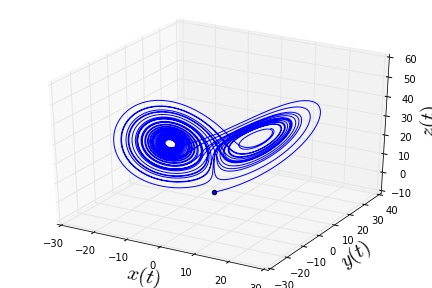
\includegraphics[scale=0.44]{lorenz_attractor.jpg}
	\label{fig:sub1}
	}
	\hfill
\subfloat[Time- domain graph for the Lorenz attractor]{
	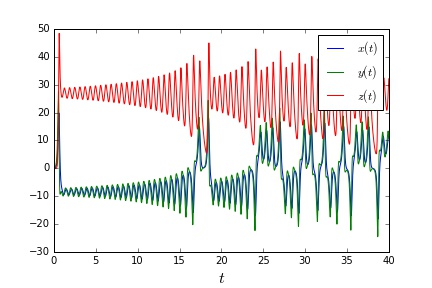
\includegraphics[scale=0.44]{lor_time_displacements.jpg}
	\label{fig:sub2}
	}
\end{figure}

Figure 5(A) shows that the curve starts near the origin $(0,0,0)$ and then begins to move into a more regular trajectory, which appears to be a path over two circular shaped orbits, famously referred to as \textit{the butterfly effect}. Interestingly, in Figure 5(B), the trajectories of $x(t)$ and $y(t)$ are plotted in a very close proximity to each other, indicating that their oscillations over time are carried out without much variation to each other. However, the $z(t)$ trajectory operates for most of its time above the trajectories of $x(t)$ and $y(t)$.

\subsection*{Extension} Deterministic chaos is defined by a system with the following properties:
\begin{itemize}
\item the system is \textit{irregular}, that is, it is aperiodic.
\item simulating the system twice using the same initial conditions will lead to the same final state. However, a slight change in initial conditions will lead to wildly different final states. Thus, the system is \textit{deterministic}.
\item the system is \textit{ordered} in the phase space.
\end{itemize}Consequently, predictions are very difficult, and near impossible, to make about the final state of a deterministically chaotic system, and these systems are associated with \textit{fractal structures}.$^{[5]}$

Chaos occurs heavily in the study of meteorology and the prediction of weather systems. Since weather behaviour can be expressed through many different factors, including thermodynamics, radiation and fluid dynamics, the equations derived from these factors are very sensitive to initial conditions, which makes long- term weather prediction very complicated. 

In weather modelling, super computers are tasked with running many simulations of the chaotic system by implementing varying initial conditions on the equations. The simulations are then studied for the likelihood of occurance. The computer simulation models can be made more accurate by including more parameters to make the model more realistic, but this is at detriment to simulation speed. A balance between simulation speed and accuracy must be balanced so that the outcomes of the weather prediction models are both accurate to a helpful degree, and completed in time to be of use to scientists and the general public, since weather predictions are only accurate for a few days into the future.$^{[6]}$

Throughout my studies of the Van der Pol oscillator, and nonlinear dynamical systems in general, it has been quite a surprise that such a rich area of mathematics exists behind equations that have no analytical solutions. It appears that, just like real world problems, the qualitative results of these dynamical systems are instrumental in gaining more meaningful and accurate insight into fundamental systems that we interact with in our daily lives.

\newpage
\section{References}

[1]	Tsatsos.M. (2006), \textit{Theoretical and Numerical Study of the Van der Pol equation}.[online]. Thessaloniki. Aristotle University of Thessaloniki. Available from: https://ipfs.io/ipfs/QmfXH\\9XtP7xmoTH8WAp4HNSduqWMwLTH8B8T\\vbTkdgzNAa/cc-by-nc-sa-3.0/0803/0803.1658.pdf [Accessed $15^\text{th}$ November 2015].

[2]	Azarkhalili.B, Moghadas.P, Rasouli.M. (2011), \textit{Approximation Behavior of Van der Pol Equation: 
Large and Small Nonlinearity Parameter}.[online]. Tehran, Iran. Sharif University of Technology. Available from: http://www.iaeng.org/publication\\/IMECS2011/IMECS2011\_pp1539-1544.pdf [Accessed $15^{\text{th}}$ November 2015].

[3]	Tallinn University (1999), \textit{Li\'enard Systems}.[online] Tallinn, Estonia. Tallinn University. Available from: http://minitorn.tlu.ee/~jaagup/uk/dynsys/ds2/limit/Lienard/Lienard.html [Accessed $15^\text{th}$ November 2015].

[4]	alunw.freeuk.com ($7^{\text{th}}$ July 2008), \textit{Chaos Theory and Strange Attractors}.[online]. Available from: http://www.alunw.freeuk.com/chaos.html [Accessed $14^{\text{th}}$ July 2001].

[5]	Nikoli\'c. K. N (2011), \textit{Introduction to Deterministic Chaos}.[online]. University of Delaware. Available from: http://www.physics.udel.edu/~bnikolic/teaching/phys660/lectures/\\deterministic\_chaos.pdf [Accessed $15^\text{th}$ November 2015].

[6]	University of Birmingham (2015), \textit{Examples of Chaotic Systems}.[online] Birmingham. University of Birmingham. Available from: http://www.birmingham.ac.uk/schools/chemical-\\engineering/weblab/Introduction-to-Chaos/Examples-of-Chaotic-Systems/index.aspx [Accessed $15^\text{th}$ November 2015].
\end{document} 




